\documentclass[a4paper, 14pt]{extarticle}

\usepackage[T2A]{fontenc} % поддержка русских букв
\usepackage{cmap} % копирование и поиск по русскому тексту
\usepackage[utf8]{inputenc}
\usepackage[english, russian]{babel}

% sub figures / grids of pictures
\usepackage{subcaption} 
\usepackage{graphicx}
\graphicspath{{../img/}} % includegraphics path
\newcommand{\includegraphicsw}[2][1.]{\includegraphics[width=#1\linewidth]{#2}}
% pdf
\usepackage{pdfpages}
% tables
\let\oldtabular\tabular
\renewcommand{\tabular}[1][1.5]{\def\arraystretch{#1}\oldtabular}
\usepackage{multirow}
\usepackage{colortbl}
% \coloneqq
\usepackage{mathtools}
\usepackage{amssymb}
% math commands for convinience
\DeclareMathOperator{\argmin}{arg\,min}
% bold vectors
\newcommand{\vect}[1]{\boldsymbol{\mathbf{#1}}}

\begin{document}
	%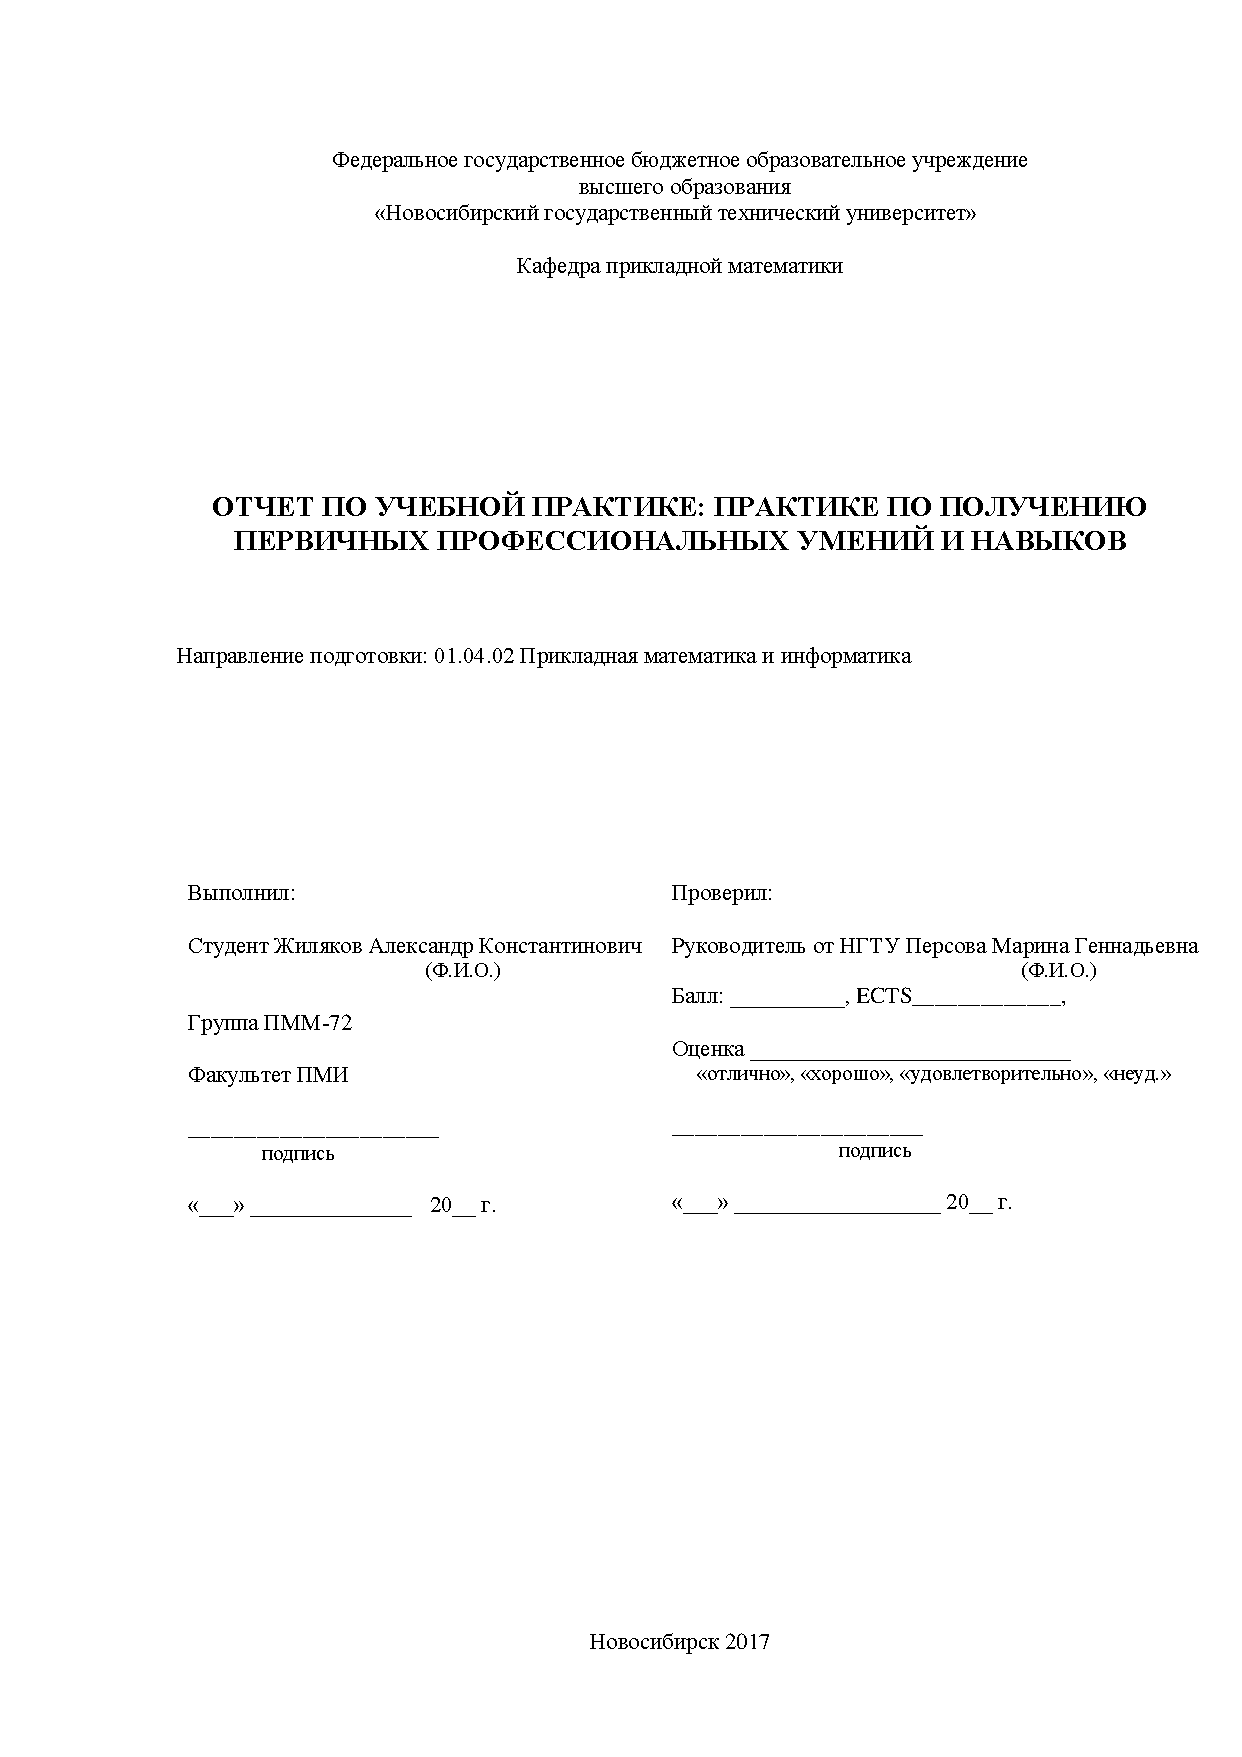
\includepdf{title.pdf}
	%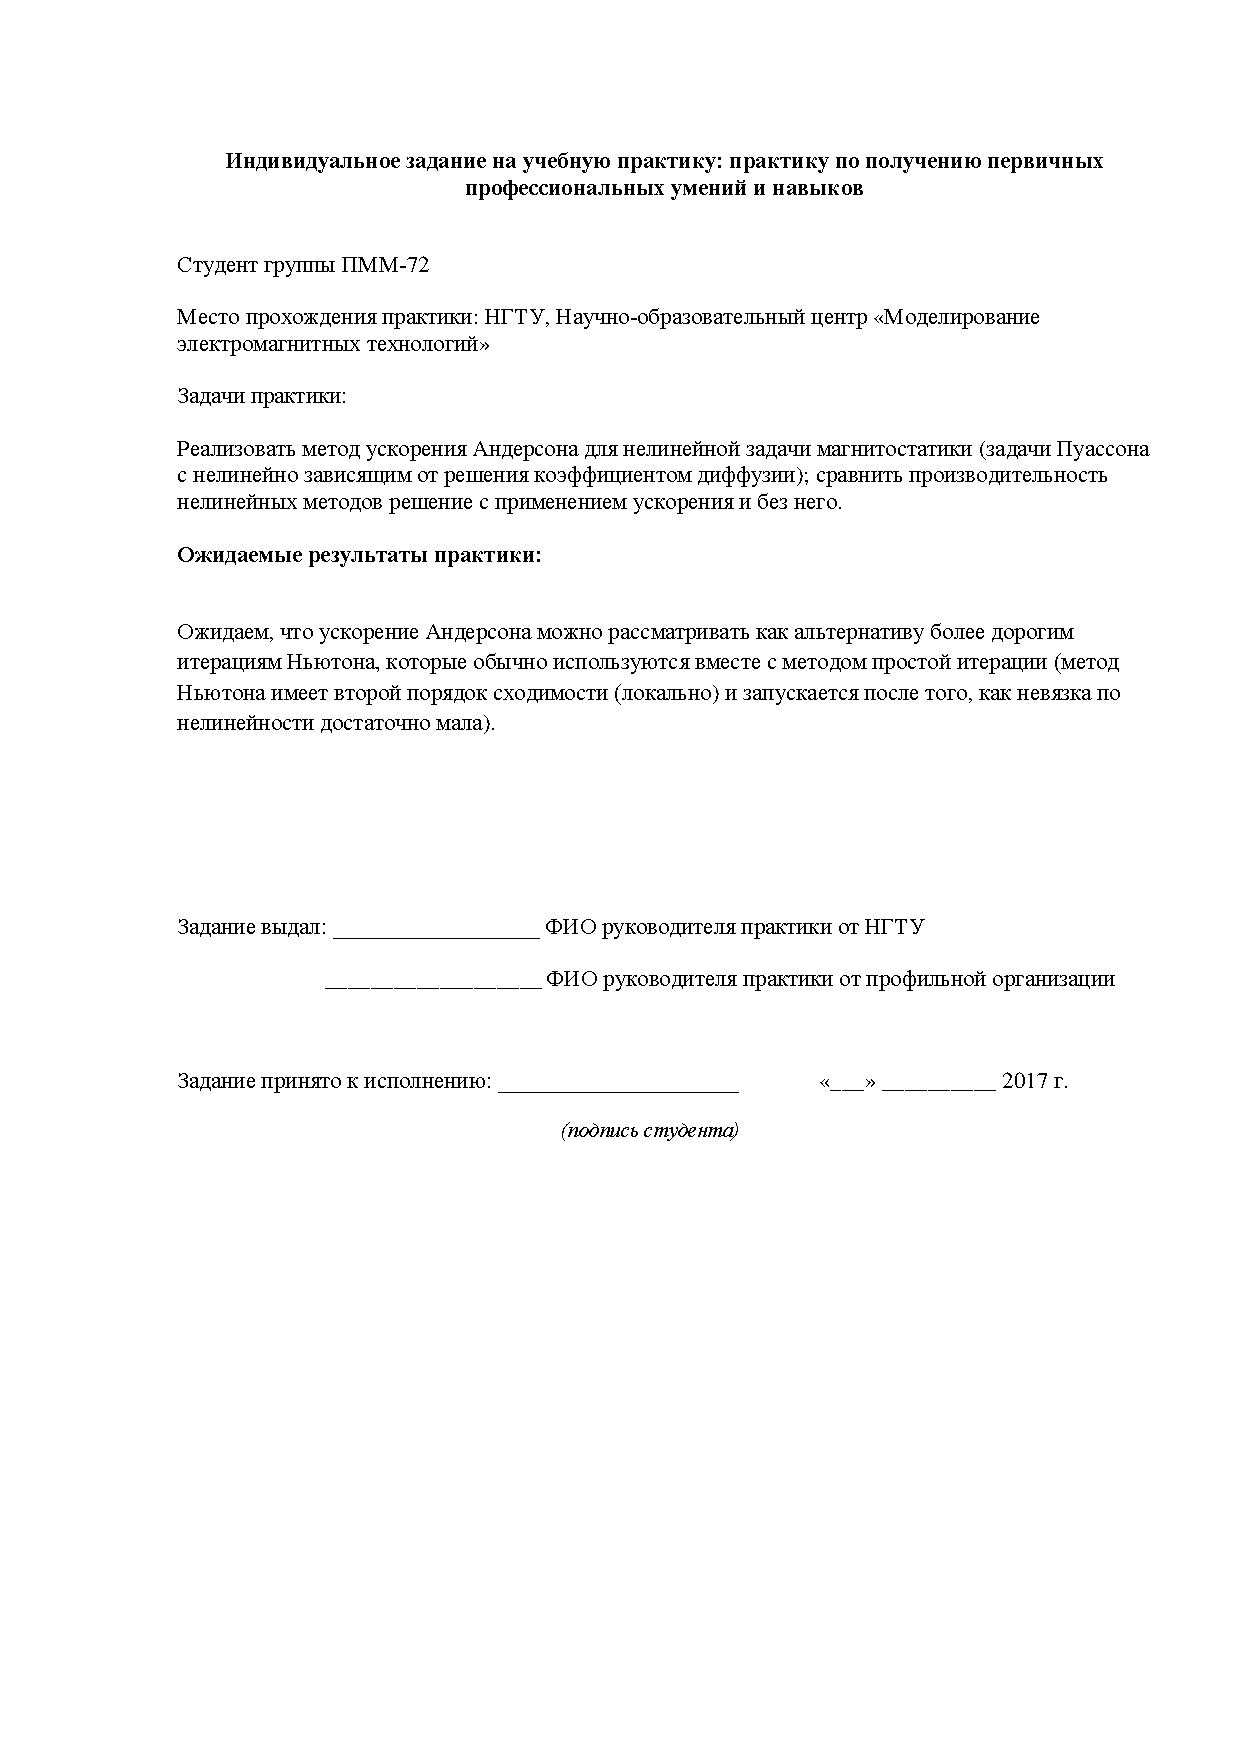
\includepdf{todo.pdf}
	
	\section{Описание задачи}
	
	\begin{figure}[b!]
		\centering
		\includegraphicsw[.6]{magnet.png}
		\caption{Сечение в плоскости $x\,O\,y$: железный магнит (выделен серым цветом), медные провода (выделены красным и синим)}
		\label{fig:magnet}
	\end{figure}
	
	Расчётная область представлена на рисунке~\ref{fig:magnet}. При заданной плотности тока $\vect J = (0, 0, J_z)$, $J_z \coloneqq \pm j \left[A\,m^{-2}\right]$ в проводах и магнитной проницаемости $\mu \left[N\,A^{-2}\right]$ железного тела, требуется найти результирующее поле магнитной индукции $\vect B \left[T\right]$.
	
	Физика данной задачи описывается системой Максвелла. Введём в рассмотрение вектор-потенциал~$\vect A$ через 
	$$
		\vect B = \nabla\times\vect A;
	$$
	тогда уравнения Максвелла $\nabla\times\frac{1}{\mu} \vect B = \vect J$, $\nabla\cdot\vect B = 0$ можно переписать в терминах вектор-потенциала
	$$
		\nabla\times\frac{1}{\mu}\nabla\times\vect A = \vect J.
	$$
	Предполагая, что магнит достаточно длинный в $z$-направлении и учитывая тот факт, что поле $\vect J$ имеет только одну ненулевую $z$-компоненту, $J_z = J_z(x, y)$, мы можем свести последнее уравнение к уравнению Пуассона
	\begin{equation}\label{poisson}
		-\nabla\cdot(\frac{1}{\mu}\nabla A_z) = J_z;
	\end{equation}
	из физических соображений задача~\eqref{poisson} оснащается однородными краевыми условиями Неймана (на нижней границе) и Дирихле (на остальной части). В результате КЭ-дискретизации задача сведётся к решению линейной
	\begin{equation}\label{linear}
		\vect S\,\vect x = \vect b
	\end{equation}
	или нелинейной
	\begin{equation}\label{nonlinear}
		\vect S(\vect x)\,\vect x = \vect b
	\end{equation}
	системе уравнений в зависимости от того, каким образом магнитная проницаемость зависит от вектор-потенциала. 
	
	Представим магнитную проницаемость в виде $\mu = \mu_0\,\hat\mu$, где $\mu_0 \coloneqq 4\,\pi\,10^{-7} \left[N\,A^{-2}\right]$ есть проницаемость вакуума. Мы можем положить $\hat\mu_{\text{iron}} = 1000$ --- тогда~\eqref{poisson} сведётся к линейной системе~\eqref{linear}. В таком случае ... (описать скейлинг и метод решения слау)
	
	В действительности же $\hat\mu_{\text{iron}}$ нелинейно зависит $\vect B$ (см. рисунок~\ref{mu}) --- $\mu_{\text{iron}} = \mu_{\text{iron}}(||\vect B|| = ||\nabla A_z||)$. При таком раскладе~\eqref{poisson} сведётся к нелинейной системе~\eqref{linear}. Далее мы рассмотрим методы решения нелинейных систем. 
	
	\begin{figure}[b!]
		\centering
		\begin{subfigure}{.45\linewidth}
			\centering
			\includegraphicsw{interp.pdf}
			\caption{$\hat\mu_{\text{iron}} = \hat{\mu}_{\text{iron}}(||\vect B||)$}
		\end{subfigure}%
		\hfill
		\begin{subfigure}{.45\linewidth}
			\centering
			\includegraphicsw{extrap.pdf}
			\caption{Часть с экстраполяцией}
		\end{subfigure}
		\caption{Интерполянт для магнитной проницаемости, построенный по реальным данным}
		\label{mu}
	\end{figure}
	
	\section{Ускорение Андерсона}
	
	Пусть требуется решить нелинейную задачу
	\begin{equation}\label{f}
		\vect f(\vect x) = 0.
	\end{equation}
	От задачи поиска корня~\eqref{f}, записанной в терминах оператора невязки~$\vect f : \mathbb R^n \rightarrow \mathbb R^n$, можно перейти к эквивалентвной задаче поиска фиксированной точки
	\begin{equation}\label{g}
		\vect x = \vect g(\vect x),
	\end{equation}
	записанной в форме оператора итераций~$\vect g$. (Сделать это можно, например, положив~$\vect g(\vect x) \coloneqq \vect x - \gamma\,f(\vect x)$.)
	
	Выбрав начальное приближение~$\vect x^{(0)}$, для решения~\eqref{g} можно применить \textbf{метод простой итерации}
	\begin{equation}\label{fp}
		\vect x^{(k+1)} = \vect g(\vect x^{(k)}).
	\end{equation}
	
	Для ускорения сходимости~\eqref{fp} можно предложить следующую идею. Будем искать новое приближения, используя $(m + 1)$ предыдущих приближений:
	\begin{equation}\label{am1}
		\vect x^{(k+1)} = \sum_{i=0}^m \alpha_i\,\vect g(\vect x^{(k-i)}).
	\end{equation}
	Метод~\eqref{am1} будет состоятельным тогда и только тогда, когда 
	\begin{equation}\label{am2}
		\sum_{i=0}^m \alpha_i = 1.
	\end{equation}
	Коэффициенты~$\alpha_i$ будем искать, решая задачу минимизации
	\begin{equation}\label{am3}
		\vect\alpha = \underset{\sum_{i=0}^m \alpha_i = 1}{\argmin} \left\lVert \sum_{i=0}^m \alpha_i\,\vect f(\vect x^{(k-i)}) \right\lVert_2.
	\end{equation}
	
	Представим коэффициенты~$\alpha_i$ в виде
	\begin{align*}
		\alpha_0		&= 1 - \beta_1, \\
		\alpha_1		&= \beta_1 - \beta_2, \\
		\vdots			& \\
		\alpha_{m-1}	&= \beta_{m-1} - \beta_m, \\
		\alpha_m		&= \beta_m;
	\end{align*}
	тогда задачу минимизации с ограничениями~\eqref{am3} можно переписать как задачу минимизации без ограничений --- задаче наименьших квадратов
	\begin{equation}\label{lsq}
		\begin{aligned}
			\vect\beta 
				&= \underset{\vect\beta \in \mathbb R^m}{\argmin} \left\lVert \vect f(\vect x^{(k)}) - \sum_{i=1}^{m} \beta_i\,(\vect f(\vect x^{(k-i)}) - \vect f(\vect x^{(k-i+1)})) \right\lVert_2 \\
				&= \underset{\vect\beta \in \mathbb R^m}{\argmin} \left\lVert \vect f(\vect x^{(k)}) - \vect F\,\vect\beta \right\lVert_2, \\
			\left(\vect F^T\,\vect F\right)\,\vect\beta 
				&= \vect F^T\,\vect f(x^{(k)}), \text{ где} \\ 
			\vect F 
				&\coloneqq \begin{pmatrix}
					\vect f(\vect x^{(k)} - \vect f(\vect x^{(k-1)}) & \dots & \vect f(\vect x^{(k-m+1)} - \vect f(\vect x^{(k-m)})
				\end{pmatrix} \in \mathbb R^{m \times n}.
		\end{aligned}
	\end{equation}
	
	\section{Численные результаты}
	
\end{document}


